\section{Introduction}

\begin{frame}
\frametitle{Electronic Systems Design}
\begin{block}{The focus is on the {\bfseries system}}
A system is a set of interacting {\em components} that form a whole
\end{block}
\pause
\begin{exampleblock}{The design is {\bfseries simplified} by focusing on components}
The team designing one component needs to have minimum knowledge of the remaining system
\end{exampleblock}
\pause
\begin{alertblock}{To make components interact requires {\bfseries collaboration}}
Teams need to exchange information and specifications in an efficient/effective way
\end{alertblock}
\end{frame}

\begin{frame}
\frametitle{Objectives}
\begin{enumerate}
\item Become familiar with tools that facilitate team collaboration
\item Acquire expertise in design techniques for large projects
\item Learn a programming language for the design of digital electronic systems
\end{enumerate}
\end{frame}

\begin{frame}
\frametitle{What's new in this course?}
\begin{enumerate}
\item A focus on interaction between teams
\item Software engineering methodologies for effective design
\item SystemC as the design language
\end{enumerate}
\end{frame}

\begin{frame}
\frametitle{What are we supposed to know already?}

{\small
\begin{block}{C++ programming}
This is necessary since SystemC is a C++ library. We will quickly review object-oriented design.
\end{block}
\begin{block}{VHDL programming}
This is useful for SystemC programming, because the approach is very similar.
\end{block}
\begin{block}{UML}
While we will briefly repeat the most useful diagrams, some previous experience helps.
\end{block}
\begin{block}{Use of a *nix OS}
The reference platform will be Linux, with OSX working almost in the same way; Windows, while usable, is a bit less practical.
\end{block}
}
\end{frame}

\section{Topics}

\subsection{Team Interaction}

\begin{frame}
\frametitle{Team interaction}
\framesubtitle{Summary}
\begin{enumerate}
\item Use the Unified Modeling Language (UML) to document and exchange specifications
\item Use a distributed version control system (DVCS) to be able to exchange code reliably
\item Use an issue tracking system (ITS) to manage in-project and cross-project problems
\item Use an automated build system for reproducibility among teams
\end{enumerate}
\end{frame}

\begin{frame}
\frametitle{Team interaction}
\framesubtitle{Tools - 1}
\begin{block}{UML}
\begin{itemize}
\item Violet: \url{http://alexdp.free.fr/violetumleditor/page.php} \,\,\, (cross-platform) (recommended)
\item Dia: \url{https://live.gnome.org/Dia} (cross-platform)
\item LucidChart: \url{https://www.lucidchart.com} \,\,\, (web-based)
\end{itemize}
\end{block}

\begin{block}{Version Control}
\begin{itemize}
\item Git: \url{http://git-scm.com} \,\,\, (cross-platform)
\end{itemize}
\end{block}

\end{frame}

\begin{frame}
\frametitle{Team interaction}
\framesubtitle{Tools - 2}

\begin{block}{Issue Tracking}
\begin{itemize}
\item BitBucket: \url{https://bitbucket.org} \,\,\, (web-based)
\end{itemize}
\end{block}

\begin{block}{Build Automation}
\begin{itemize}
\item CMake: \url{http://cmake.org} \,\,\, (cross-platform)
\end{itemize}
\end{block}

\end{frame}

\begin{frame}
\frametitle{Team interaction}
\framesubtitle{Book resources}
\begin{itemize}
\item R. Miles, K. Hamilton, "Learning UML 2.0", O'Reilly (2006)
\item J. Loeliger, M. McCullough, "Version Control with Git", O'Reilly (2012)
\item K. Martin, B. Hoffman, "Mastering CMake", Kitware Inc. (2010)
\end{itemize}
\end{frame}

\begin{frame}
\frametitle{Team interaction}
\framesubtitle{Online resources}
\begin{enumerate}
\item \url{http://edn.embarcadero.com/article/31863}
\item \url{http://git-scm.com/book}
\item \url{https://confluence.atlassian.com/display/BITBUCKET/Using+your+Bitbucket+Issue+Tracker}
\item \url{http://www.cmake.org/cmake/help/cmake_tutorial.html}
\end{enumerate}
\end{frame}

\subsection{Software engineering}

\begin{frame}
\frametitle{Software engineering}
\framesubtitle{Summary}

\begin{enumerate}
\item Learn to write self-documenting code before relying on comments
\item Adopt the {\em Test Driven Development} approach to coding
\item Write code first, then {\em refactor} to clean up your mess
\item (optional) Exploit an Integrated Development Environment (IDE) for refactoring and debugging
\end{enumerate}

\end{frame}

\begin{frame}
\frametitle{Software engineering}
\framesubtitle{Tools}
\begin{block}{Integrated Development Environment}
\begin{itemize}
\item KDevelop: \url{http://www.kdevelop.org} \,\,\, (cross-platform) (recommended)
\item Eclipse: \url{http://eclipse.org} \,\,\, (cross-platform)
\item Visual Studio 2012: \url{http://www.microsoft.com/visualstudio/eng} \,\,\, (windows, commercial)
\end{itemize}
\end{block}
\end{frame}

\begin{frame}
\frametitle{Software engineering}
\framesubtitle{Resources}
\begin{block}{Books}
\begin{enumerate}
\item R. Martin, "Clean Code", Prentice Hall (2008)
\item K. Beck, "Test Driven Development", Addison-Westley (2002)
\item M. Fowler, K. Beck, J. Brant, W. Opdyke, "Refactoring", Addison-Westley (1999)
\end{enumerate}
\end{block}

\begin{block}{Online}
\begin{enumerate}
\item \url{http://c2.com/cgi/wiki?SelfDocumentingCode}
\item \url{http://www.agiledata.org/essays/tdd.html}
\item \url{http://sourcemaking.com/refactoring}
\end{enumerate}
\end{block}

\end{frame}

\subsection{SystemC programming}

\begin{frame}
\frametitle{SystemC programming}
\framesubtitle{Summary}

\begin{itemize}
\item Learn to describe a component using models at different levels of abstraction
\item Perform tests on a component in isolation or when communicating with components from other teams
\end{itemize}

\pause
\begin{block}{Synthesis will not be covered}
Testing will be performed at the code level only.
\end{block}
\end{frame}

\begin{frame}
\frametitle{SystemC programming}
\framesubtitle{Tools}

\begin{block}{The library itself}
\begin{itemize}
\item SystemC: \url{http://www.accellera.org/downloads/standards/systemc} \,\,\, (cross-platform) (requires free registration)
\end{itemize}
\end{block}

\end{frame}

\begin{frame}
\frametitle{SystemC programming}
\framesubtitle{Resources}
\begin{block}{Books}
\begin{itemize}
\item D. Black, J. Donovan, B. Bunton, A. Keist, \\  "SystemC: from the ground up", Springer (2010)
\end{itemize}
\end{block}

\begin{block}{Online}
\begin{enumerate}
\item \url{http://www.asic-world.com/systemc/tutorial.html}
\item \url{http://www.doulos.com/knowhow/systemc/tutorial}
\item \url{http://www.ht-lab.com/howto/vh2sc_tut/vh2sc_tut.html}
\end{enumerate}
\end{block}

\end{frame}

\section{Organization}

\begin{frame}
\frametitle{Organization of the course}
\framesubtitle{Summary}
\begin{enumerate}
\item Modeling with UML: theory and some practice
\item Version control with Git: theory and practice
\item Issue tracking with BitBucket: some theory, mainly practice
\item Build automation with CMake: mainly practice
\item C++ basics: theory and practice
\item Design with SystemC: theory and practice
\item Design of a System-on-Chip (SoC) with SystemC: practice only
\end{enumerate}
\end{frame}

\begin{frame}
\frametitle{Organization of the course}
\framesubtitle{Design of a System-on-Chip}

\begin{block}{What is a System-on-Chip?}
An SoC is an integrated circuit that includes all the necessary components of a computer within a single package.
\end{block}
\pause
\begin{block}{What does it include?}
Essentially anything:
\begin{itemize}
\item Processing (analog or digital)
\item Storage (volatile or persistent)
\item Voltage regulation for internal components
\end{itemize}
\pause
\end{block}
\begin{block}{What do we need to build a computer?}
Very little: with proper buffering/amplification/matching, you can just wire the SoC pins to external I/O ports and to the power supply.
\end{block}
\end{frame}

\begin{frame}
\frametitle{Organization of the course}
\framesubtitle{Example of a SoC (from Wikipedia)}
\begin{figure}
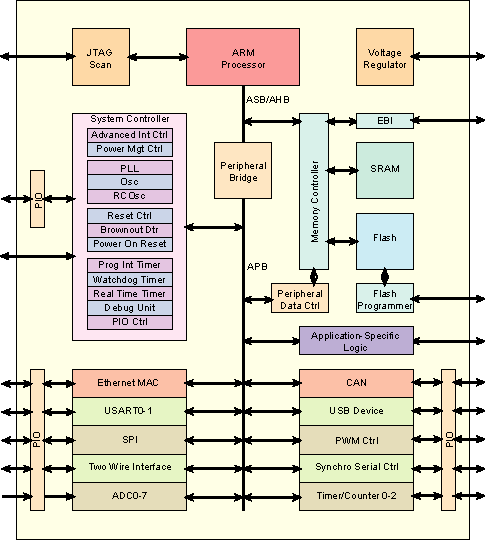
\includegraphics[width=0.7\textwidth]{lecture01/img/ARMSoCBlockDiagram.png}
\end{figure}
\end{frame}

\begin{frame}
\frametitle{Organization of the course}
\framesubtitle{How to develop "our" SoC}
\begin{block}{We split the development into a number of (one student) teams}
\begin{itemize}
\item The student has the exclusive responsibility of a component
\item A component may be completed or held back to focus on another new component
\item If necessary, responsibility of a component may be passed on to another student
\end{itemize}
\end{block}
\pause
\begin{block}{There is no particular focus on achievements}
We are not supposed to complete the project within the limited hours allowed for the course. There is more
focus on methodology than results.
\end{block}

\end{frame}

\section{Exam}

\begin{frame}
\frametitle{The examination}
\framesubtitle{Summary}
\begin{block}{Project report}
Each student must deliver a report at least 24 hours before the exam in electronic format by email. This is mandatory to gain access to the oral exam.
\end{block}

\begin{block}{Oral}
It will involve discussion of the project report. Additional
oral/written questions will complete the examination. Duration: between 10 and 20 minutes.
\end{block}

\end{frame}

\begin{frame}
\frametitle{The examination}
\framesubtitle{Project report}

\begin{block}{What to put into it}
\begin{itemize}
\item Describe the activities performed, with UML diagrams and code snippets where necessary
\item Describe your interaction with other students
\item Create a timeline of your development on the repository
\item Make specific mentions to issues both solved and still opened
\end{itemize}
\end{block}

\end{frame}

\begin{frame}
\frametitle{The examination}
\framesubtitle{Oral}

\begin{block}{Topics covered}
\begin{itemize}
\item UML
\item Git usage
\item CMake usage
\item Issue tracking usage
\item Object-oriented design in C++
\item SystemC programming
\end{itemize}
\end{block}

\end{frame}